%\newpage
\section{Casi d'uso}
Questa sezione elenca le funzionalità offerte da \progetto\ descritte attraverso il linguaggio \gloss{UML}. 

\progetto\ può essere visto come l'insieme di più sottosistemi che verranno di seguito elencati e che sono stati descritti in modo molto generale anche attraverso la figura \ref{fig:butterfly}.
	
	\subsection{Attori}
	\begin{itemize}
		\item Redmine/GitLab
		\item Producer
		\item Utente non acceduto
		\item Utente (acceduto), il quale interagisce col gestore personale
		\item Consumer
		\item Telegram/e-mail
	\end{itemize}
	
	\subsection{Elenco casi d'uso}

%TODO: da ricordarsi: se qualcuno è offline, c'è la possibilità che il messaggio venga perso.

\newcounter{uccount}

\stepcounter{uccount}
\subsubsection{UC\theuccount\ - Redmine/GitLab invia una segnalazione}
    \begin{figure}[H]
		\centering
		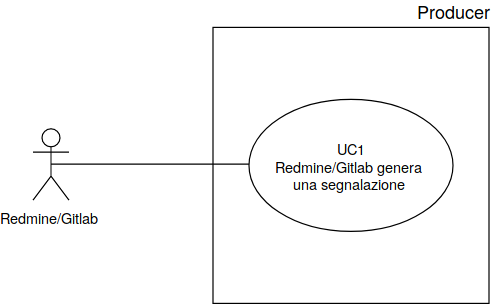
\includegraphics[width=0.7\textwidth]{img/UC1.png}\\
		\caption{UC\theuccount - Redmine/GitLab invia una segnalazione}
	\end{figure}
	\begin{itemize}
		\item \textbf{Codice}: UC\theuccount.
		\item \textbf{Titolo}: Redmine/GitLab invia una segnalazione.
		\item \textbf{Attori primari}: Redmine/Gitlab.
		\item \textbf{Descrizione}:
		 il sistema qui è il Producer ed è interno al sistema \progetto.
		 L'invio di una segnalazione avviene da parte di Redmine/GitLab in seguito all'apertura di una issue o di un commit.		 
		\item \textbf{Precondizione}: c'è qualcosa da segnalare.
		\item \textbf{Postcondizione}: segnalazione inviata.
		\item \textbf{Scenario principale}: 
		\begin{enumerate}
			\item Redmine/GitLab invia la segnalazione al Producer
		\end{enumerate}
		
	\end{itemize}

\stepcounter{uccount}
\subsubsection{UC\theuccount\ - Il Producer invia una segnalazione al Broker}
	\begin{figure}[H]
		\centering
		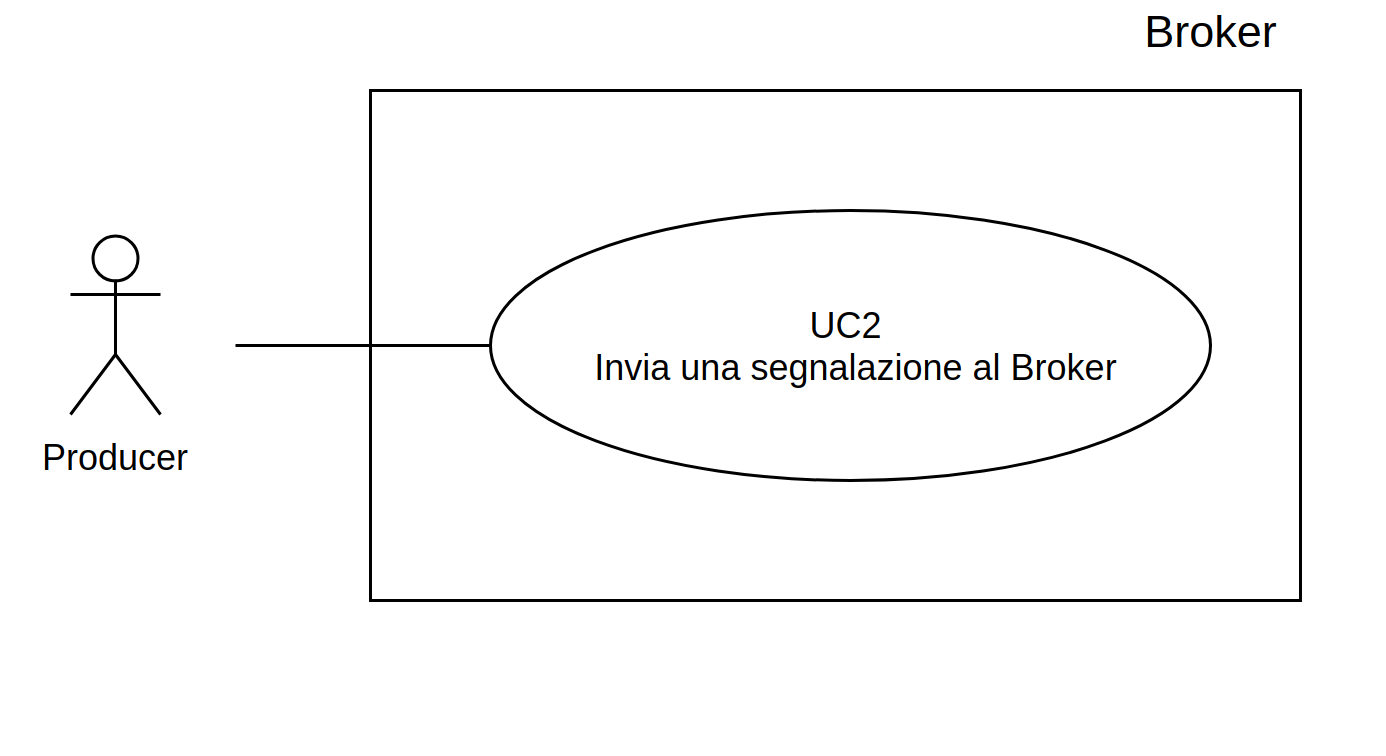
\includegraphics[width=0.9\textwidth]{img/UC2.png}\\
		\caption{UC\theuccount\ - Il Producer invia una segnalazione al Broker}
	\end{figure}
	\begin{itemize}
		\item \textbf{Codice}: UC\theuccount.
		\item \textbf{Titolo}: il Producer invia una segnalazione al Broker.
		\item \textbf{Attori primari}: Producer.
		\item \textbf{Descrizione}: il Producer, dopo aver ricevuto una determinata segnalazione da Redmine/Gitlab la inoltra al Broker. Il sistema di riferimento qui è il Broker ed è interno al sistema \progetto.
		\item \textbf{Precondizione}: il Producer ha ricevuto una segnalazione da inoltrare.
		\item \textbf{Postcondizione}: il Producer ha inviato al Broker la segnalazione.
		\item \textbf{Scenario principale}:
		\begin{enumerate}
			\item Il Producer procede all'invio della segnalazione.
		\end{enumerate}
		 
	\end{itemize}

\stepcounter{uccount}
\subsubsection{UC\theuccount\ - Il Consumer interroga il Broker}
	\begin{figure}[H]
		\centering
		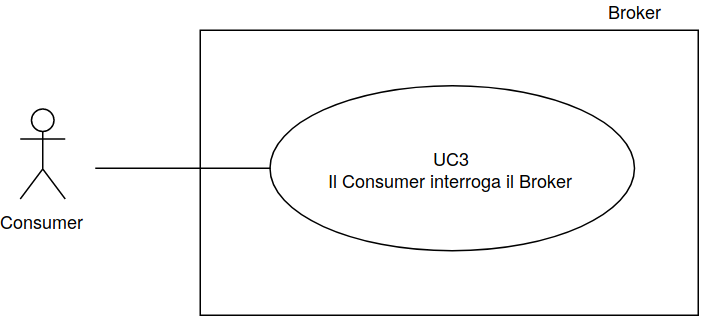
\includegraphics[width=\columnwidth]{img/UC3.png}\\
		\caption{UC\theuccount\ - Il Consumer interroga il Broker}
	\end{figure}
	\begin{itemize}
		\item \textbf{Codice}: UC\theuccount.
		\item \textbf{Titolo}: il Consumer interroga il Broker.
		\item \textbf{Attori primari}: Consumer.
		\item \textbf{Descrizione}: il Consumer chiede al Broker di acquisire il messaggio da inoltrare verso il client della tecnologia specificata dall'utente in base al Topic. Il sistema di riferimento qui è Broker ed è interno al sistema \progetto.
		\item \textbf{Precondizione}: il Broker ha un messaggio pronto ad essere inoltrato da un Consumer verso un client delle tecnologie con cui il sistema si interfaccia.
		%TODO: consumer
		\item \textbf{Postcondizione}: il messaggio recuperato dal Consumer è inoltrato al client della tecnologia correlata.
		\item \textbf{Scenario principale}: 
			\begin{enumerate}
				\item Il Consumer richiede la segnalazione da inviare al client utilizzato dall'utente finale.
			\end{enumerate}
	\end{itemize}

\stepcounter{uccount}
\subsubsection{UC\theuccount\ - Telegram/e-mail riceve un messaggio dal Consumer}
	\begin{figure}[H]
		\centering
			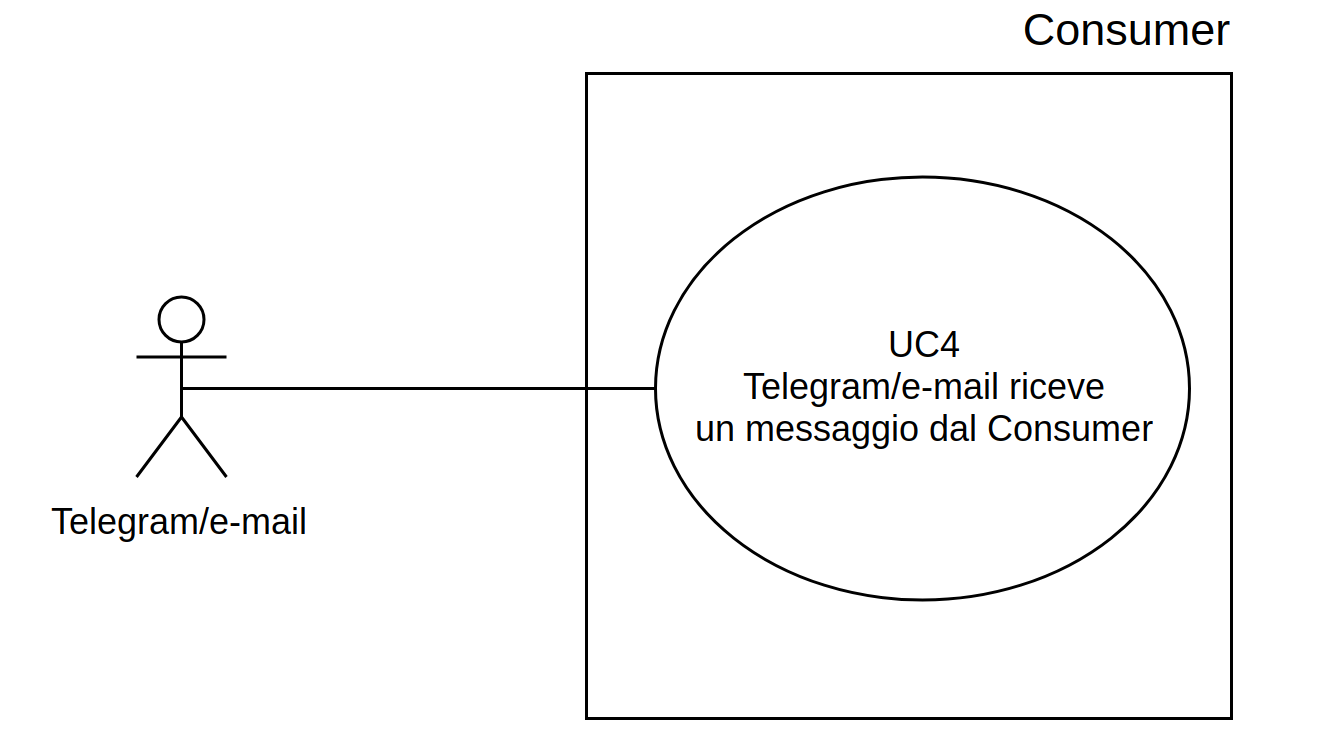
\includegraphics[width=0.7\columnwidth]{img/UC4.png}\\
		\caption{UC\theuccount\ - Telegram/e-mail riceve un messaggio dal Consumer}
	\end{figure}
	\begin{itemize}
		\item \textbf{Codice}: UC\theuccount.
		\item \textbf{Titolo}: Telegram/e-mail riceve un messaggio.
		\item \textbf{Attori primari}: Telegram/server e-mail.
		\item \textbf{Descrizione}: il sistema di riferimento qui è il Consumer ed è interno al sistema Butterfly.
		\footnote{L'\gloss{attore} Telegram/e-mail è passivo, riceve e non agisce. Viene creato questo caso d'uso al fine di inserire la funzionalità "Il Consumer invia un messaggio a Telegram/e-mail", poiché Telegram/mail è esterno a \progetto e quindi non può essere considerato un suo sottosistema.}
		
		\item \textbf{Precondizione}: il Consumer invia un messaggio a Telegram/server e-mail in seguito a un'interrogazione del Broker.
		\item \textbf{Postcondizione}: Telegram/server e-mail riceve il messaggio.
		\item \textbf{Scenario principale}:
		\begin{enumerate}
			\item La ricezione del messaggio va a buon fine.
		\end{enumerate} 
	\end{itemize}

\stepcounter{uccount}
\subsubsection{UC\theuccount\ - Accesso}
		\begin{figure}[H]
			\centering
				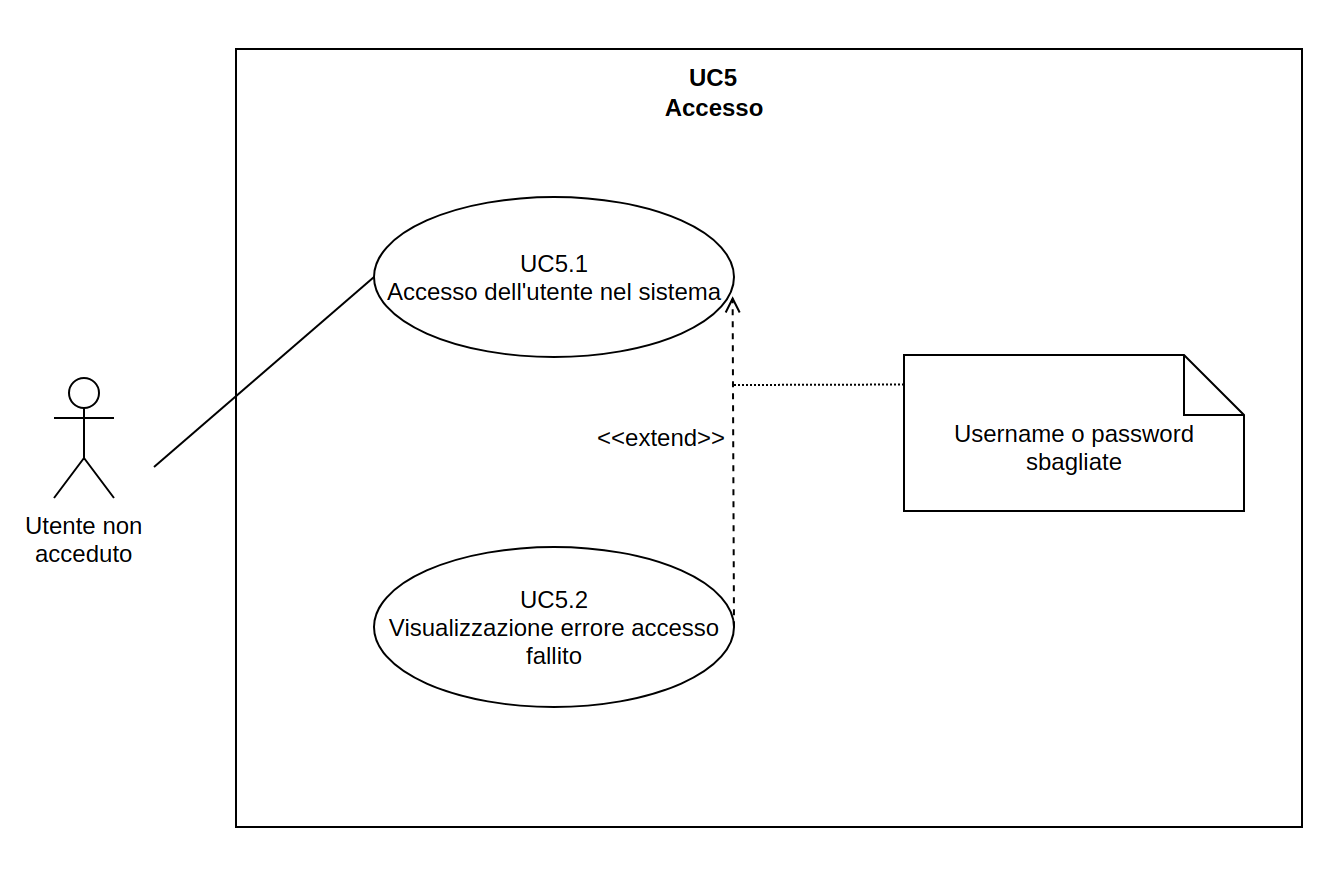
\includegraphics[width=\columnwidth]{img/UC5.png}\\
			\caption{UC\theuccount\ - Accesso}
		\end{figure}
	\begin{itemize}
		\item \textbf{Codice}: UC\theuccount.
		\item \textbf{Titolo}: accesso.
		\item \textbf{Attori primari}: utente non acceduto.
		\item \textbf{Descrizione}: l'utente richiede di accedere al sistema attraverso un form dove inserisce l'username.
		\item \textbf{Precondizione}: il sistema considera l’utilizzatore di esso come un utente non acceduto.
		\item \textbf{Postcondizione}: il sistema riconosce l'utilizzatore di esso come utente acceduto.
		\item \textbf{Scenario Principale}:
		\begin{enumerate}
			\item L'utente non ancora riconosciuto dal sistema effettua l'accesso inserendo il proprio username.
		\end{enumerate}
	\end{itemize}
	
	\paragraph{UC\theuccount.1 - Accesso dell'utente nel sistema}
		\begin{figure}[H]
			\centering
				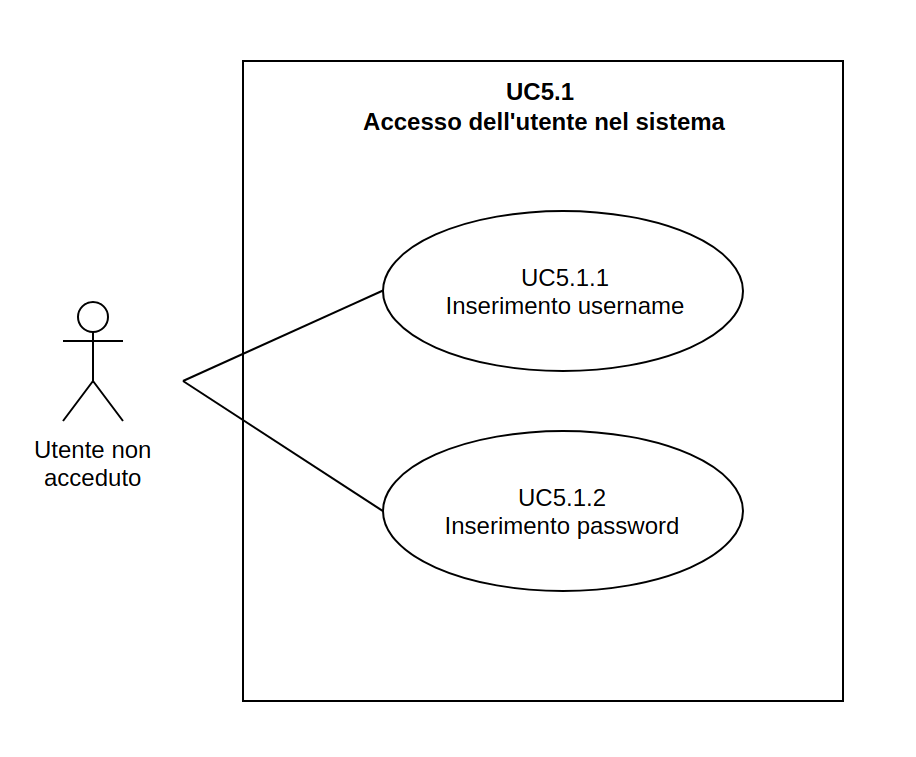
\includegraphics[width=\columnwidth]{img/UC5_1.png}\\
			\caption{UC\theuccount.1 - Accesso dell'utente nel sistema}
		\end{figure}
		\begin{itemize}
			\item \textbf{Codice}: UC\theuccount.1.
			\item \textbf{Titolo}: accesso dell'utente nel sistema.
			\item \textbf{Attori primari}: utente non acceduto.
			\item \textbf{Descrizione}: l'utente attende l'autenticazione da parte del sistema.
			\item \textbf{Precondizione}: il sistema riconosce l'utilizzatore come un utente non autenticato.
			\item \textbf{Postcondizione}: il sistema riconosce l'utente autenticato con successo.
			\item \textbf{Scenario Principale}:
			\begin{enumerate}
				\item L’utente non ancora riconosciuto dal sistema richiede l'autenticazione attraverso l'inserimento dell'username.
			\end{enumerate}
			\item \textbf{Estensioni}:
			\begin{enumerate}
				\item L'accesso non va a buon fine e viene visualizzato un errore avvisando l'utente [UC5.2].
			\end{enumerate}
	\end{itemize}

		\subparagraph{UC\theuccount.1.1 - Inserimento username}
			\begin{itemize}
				\item \textbf{Codice}: UC\theuccount.1.1
				\item \textbf{Titolo}: inserimento username.
				\item \textbf{Attori primari}: utente non acceduto.
				\item \textbf{Descrizione}: l'utente inserisce l'username.
				\item \textbf{Precondizione}: il sistema offre l'interfaccia grafica adatta all'inserimento dell'username.
				\item \textbf{Postcondizione}: l'utente ha inserito l'username desiderato.
				\item \textbf{Scenario Principale}:
				\begin{enumerate}
					\item L'utente inserisce l'username per autenticarsi.
				\end{enumerate}
			\end{itemize}
		
%		\subparagraph{UC\theuccount.1.2 - Inserimento password}
%			\begin{itemize}
%				\item \textbf{Codice}: UC\theuccount.1.2	
%				\item \textbf{Titolo}: inserimento password
%				\item \textbf{Attori primari}: utente non acceduto
%				\item \textbf{Descrizione}: l'utente inserisce la password
%				\item \textbf{Precondizione}: il sistema offre l'interfaccia grafica adatta all'inserimento della password
%				\item \textbf{Postcondizione}: l'utente ha inserito la password desiderata
%				\item \textbf{Scenario Principale}: l'utente inserisce la password per autenticarsi.
%			\end{itemize}
	
	\paragraph{UC\theuccount.2 - Visualizzazione errore autenticazione fallita}
		\begin{itemize}
			\item \textbf{Titolo}: visualizzazione errore autenticazione fallita.
			\item \textbf{Attori primari}: utente non ecceduto.
			\item \textbf{Descrizione}: l'utente viene avvisato che ha inserito username errato.
			\item \textbf{Precondizione}: il sistema riceve una richiesta di accesso da parte di un utente che
			fornisce un username errato. 
			\item \textbf{Postcondizione}: il sistema comunica all'utilizzatore l'errore.
			\item \textbf{Scenario Principale}:
			\begin{enumerate}
				\item L'utente visualizza il messaggio d'errore.
			\end{enumerate}
		\end{itemize}


\stepcounter{uccount}
\subsubsection{UC\theuccount\ - Modifica delle preferenze}
	\begin{figure}[H]
		\centering
		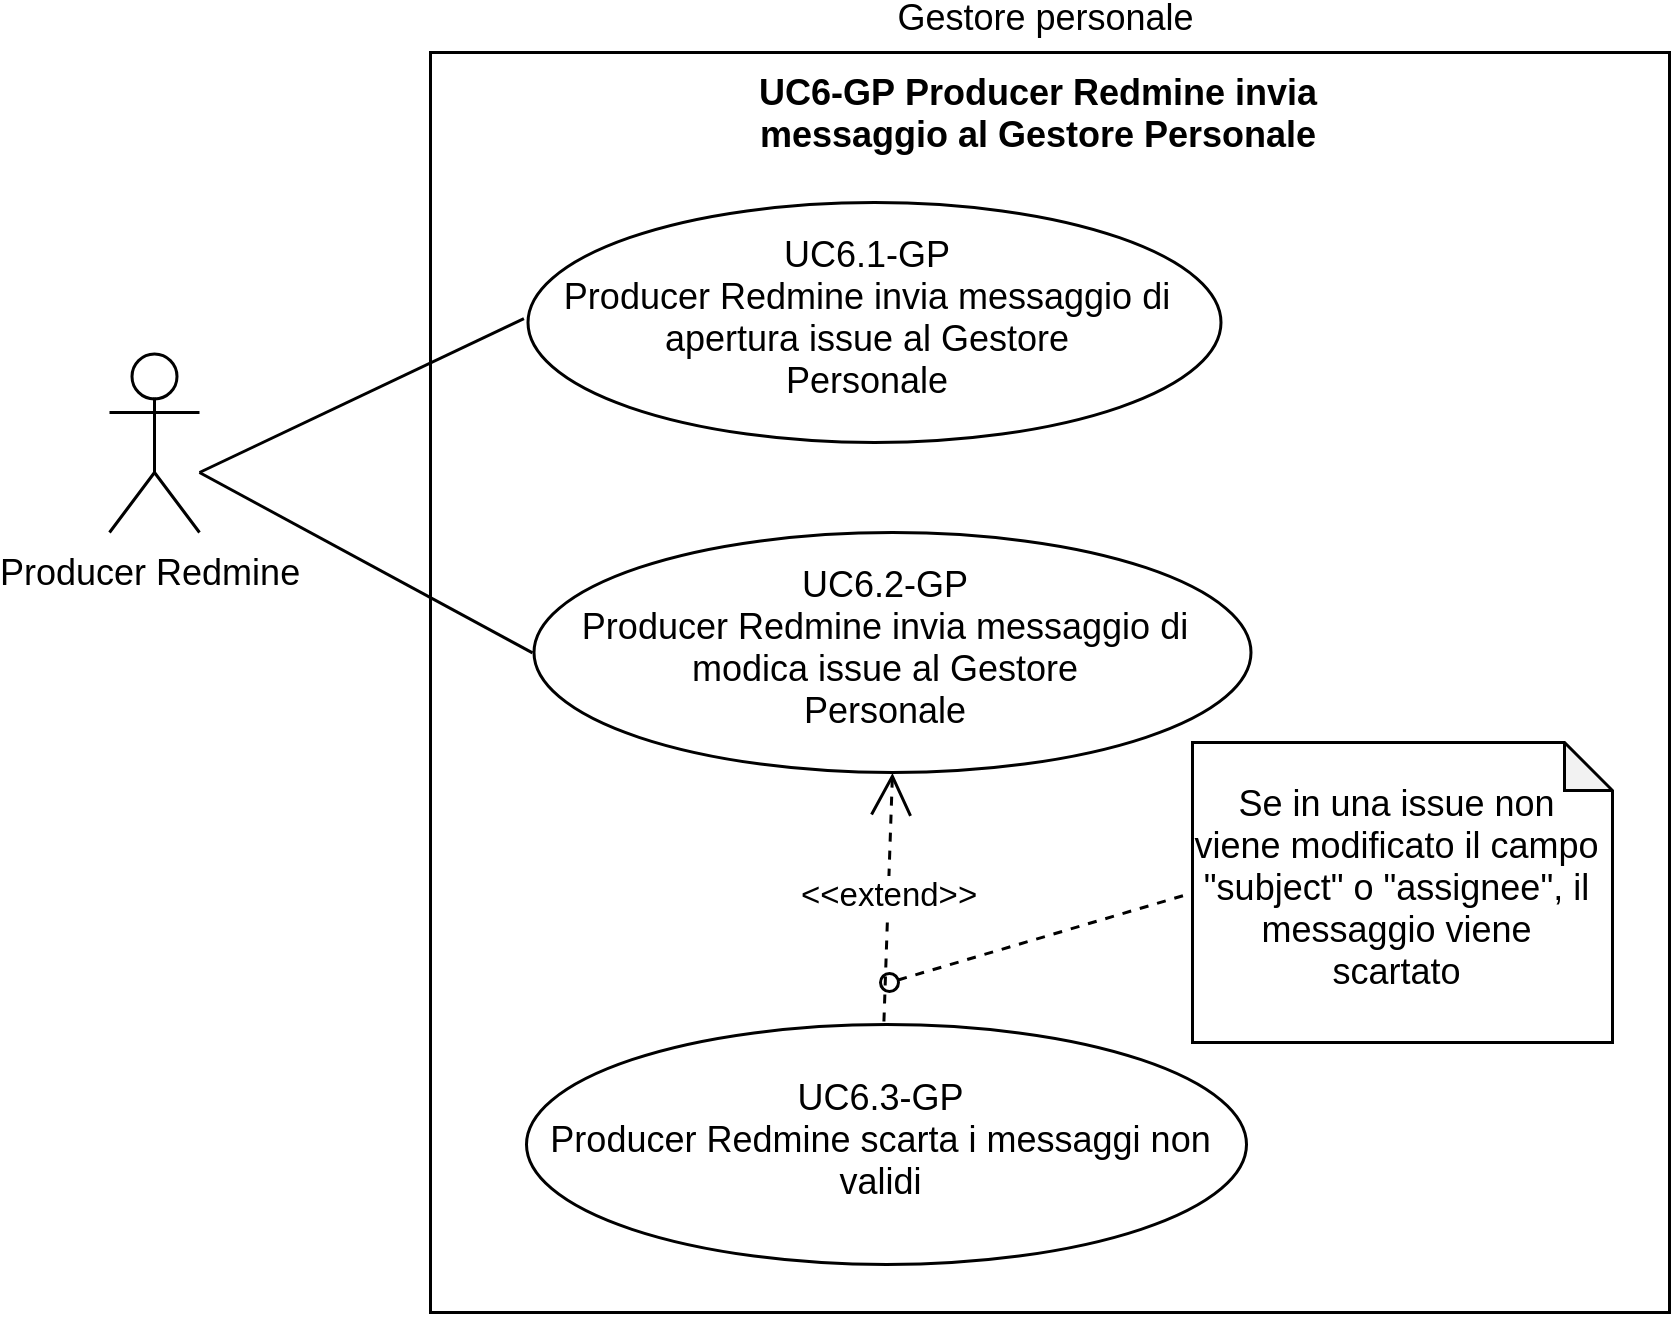
\includegraphics[width=\columnwidth]{img/UC6.png}\\
		\caption{UC\theuccount\ - Modifica delle preferenze}
	\end{figure}
	\begin{itemize}
		\item \textbf{Codice}: UC\theuccount.
		\item \textbf{Titolo}: modifica delle preferenze.
		\item \textbf{Attori primari}: utente.
		\item \textbf{Descrizione}: attraverso un'interfaccia l'utente può modificare i vari parametri per configurare l'applicazione per le proprie esigenze. Il sistema di riferimento considerato è tutto \progetto.
		\item \textbf{Precondizione}: l'utente ha acceduto con le sue credenziali corrette nel sistema.
		\item \textbf{Postcondizione}: l'utente effettua zero o più modifiche nella configurazione personale dell'applicazione. 
		\item \textbf{Scenario Principale}:
		\begin{enumerate}
			\item L'utente apporta delle modifiche alle sue preferenze all'interno dell'applicazione \progetto.
		\end{enumerate}
	\end{itemize}



	\paragraph{UC\theuccount.1 - Aggiunta preferenze}
		\begin{figure}[H]
			\centering
			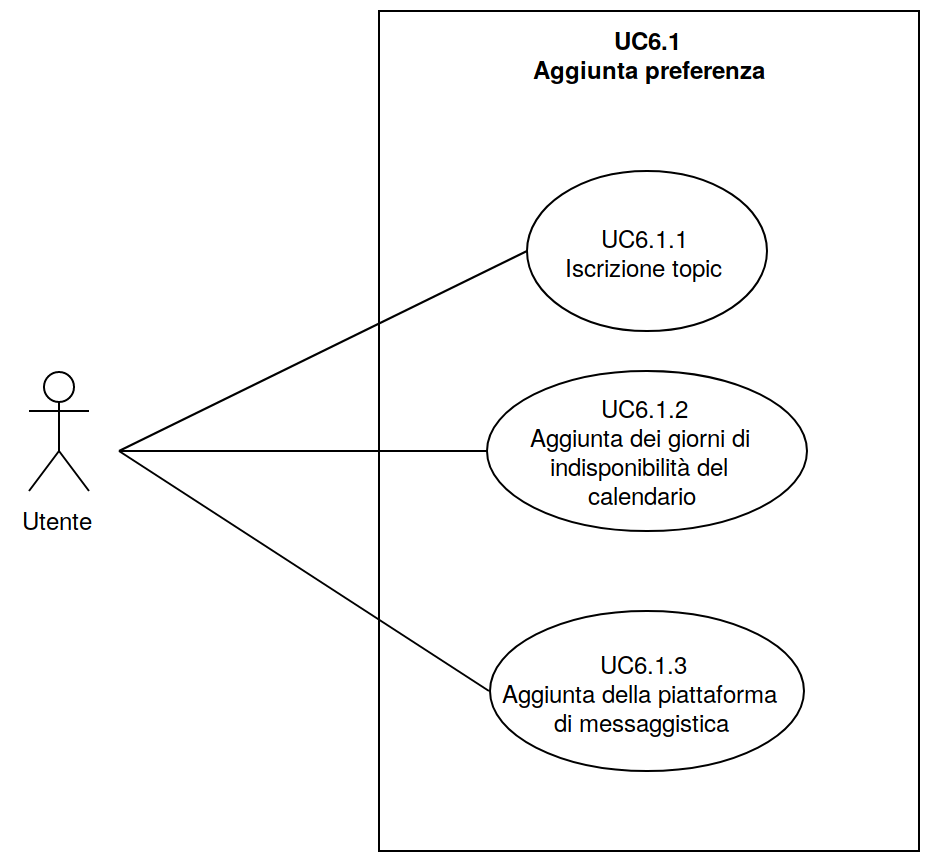
\includegraphics[width=\columnwidth]{img/UC6_1.png}\\
			\caption{UC\theuccount.1 - Aggiunta preferenze}
		\end{figure}
	\begin{itemize}
		\item \textbf{Codice}: UC\theuccount.1.
		\item \textbf{Titolo}: aggiunta preferenze.
		\item \textbf{Attori primari}: utente.
		\item \textbf{Descrizione}: l'utente, date le varie opzioni per configurare \progetto, aggiunge una preferenza tra Topic, giorni di calendario e piattaforme di messaggistica come Telegram o e-mail.
		\item \textbf{Precondizione}: l'utente ha acceduto con le sue credenziali corrette nel sistema e non ha selezionato tutte le preferenze possibili proposte da \progetto.
		\item \textbf{Postcondizione}: lo nuova configurazione contiene una o più preferenza in aggiunta rispetto alla quella precedente.
		\item \textbf{Scenario principale}: l'utente può scegliere, tra le varie opzioni disponibili disponi, quale aggiungere alla sua configurazione personale.
	\end{itemize}
	
	\subparagraph{UC\theuccount.1.1 - Iscrizione Topic}
	\begin{itemize}
		\item \textbf{Codice}: UC\theuccount.1.1.
		\item \textbf{Titolo}: iscrizione Topic.
		\item \textbf{Attori primari}: utente.
		\item \textbf{Descrizione}: data la lista di Topic presenti già inserita precedentemente, l'utente seleziona quelli a cui è interessato ricevendone una notifica. I Topic sono divisi per categoria comprendendo etichette o parole chiave stabilite in precedenza.
		\item \textbf{Precondizione}: l'utente ha acceduto con le sue credenziali corrette nel sistema e non ha selezionato tutti i Topic possibili proposti da \progetto.
		\item \textbf{Postcondizione}: il numero di Topic a cui è interessato l'utente è aumentato.
		\item \textbf{Scenario principale}:
		\begin{enumerate}
			\item L'utente aggiunge uno o più Topic dalla lista proposta dall'applicazione \progetto.
		\end{enumerate}
	\end{itemize}
		
			
	\subparagraph{UC\theuccount.1.2 - Aggiunta giorno irreperibilità nel calendario} 
	\begin{itemize}
		\item \textbf{Codice}: UC\theuccount.1.2.
		\item \textbf{Titolo}: aggiunta dei giorni di indisponibilità nel calendario.
		\item \textbf{Attori primari}: utente.
		\item \textbf{Descrizione}: dato il calendario lavorativo, l'utente aggiunge i giorni in cui non è reperibile e non vuole ricevere notifiche.
		\item \textbf{Precondizione}: l'utente ha acceduto con le sue credenziali corrette nel sistema e non ha selezionato tutti i giorni di calendario proposti da \progetto.
		\item \textbf{Postcondizione}: il numero di giorni in cui l'utente non si rende disponibile è aumentato.
		\item \textbf{Scenario principale}:
		\begin{enumerate}
			\item L'utente aggiunge le date di calendario in cui non è reperibile.
		\end{enumerate}
	\end{itemize}
			
	\subparagraph{UC\theuccount.1.3 - Aggiunta della piattaforma di messaggistica}
	\begin{itemize}
		\item \textbf{Codice}: UC\theuccount.1.3.
		\item \textbf{Titolo}:aggiunta della piattaforma di messaggistica.
		\item \textbf{Attori primari}: utente.
		\item \textbf{Descrizione}: dalla lista delle piattaforme di messaggistica l'utente aggiunge quelle da cui vuole ricevere le notifiche.
		\item \textbf{Precondizione}: l'utente ha acceduto con le sue credenziali corrette nel sistema e non ha selezionato tutte le piattaforma di messaggistica possibili proposte da \progetto.
		\item \textbf{Postcondizione}: il numero di piattaforme di messaggistica selezionate dall'utente è aumentato.
		\item \textbf{Scenario principale}:
		\begin{enumerate}
			\item L'utente aggiunge le piattaforme di messaggistica da un elenco già fornito.
		\end{enumerate} 
		%telegram: nickname e mail sono già salvati nel DB
	\end{itemize}
			



	\paragraph{UC\theuccount.2 - Rimozione preferenza}
		\begin{figure}[H]
			\centering
			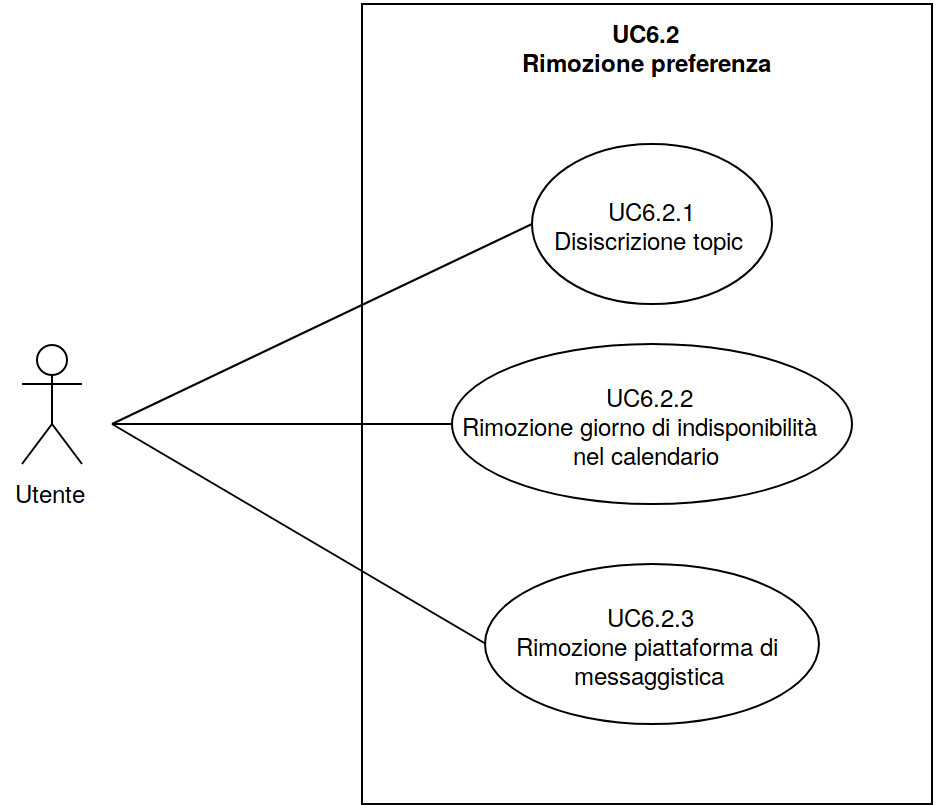
\includegraphics[width=\columnwidth]{img/UC6_2.png}\\
			\caption{UC\theuccount.2 - Rimozione preferenza}
		\end{figure}
	\begin{itemize}
		\item \textbf{Codice}: UC\theuccount.2.
		\item \textbf{Titolo}: rimozione preferenza.
		\item \textbf{Attori primari}: utente.
		\item \textbf{Descrizione}: l'utente, dopo aver selezionato delle preferenze dalle opzioni di configurazione, ne rimuove una o di più. Le preferenze consistono in Topic, date di calendario e piattaforme di messaggistica.
		\item \textbf{Precondizione}: l'utente ha acceduto con le credenziali nel sistema ed è presente almeno una preferenza selezionata tra quelle proposte da \progetto.
		\item \textbf{Postcondizione}: la nuova configurazione contiene una o più preferenze in meno rispetto a quella precedente.
		\item \textbf{Scenario principale}:
		\begin{enumerate}
			\item L'utente seleziona tra le preferenze già scelte precedentemente quale rimuovere e la toglie.
		\end{enumerate}
	\end{itemize}
	
	
	\subparagraph{UC\theuccount.2.1 - Disiscrizione Topic}
	\begin{itemize}
		\item \textbf{Codice}: UC\theuccount.2.1.
		\item \textbf{Titolo}: disiscrizione Topic.
		\item \textbf{Attori primari}: utente.
		\item \textbf{Descrizione}: l'utente di disiscrive da uno o più Topic dai quali prima riceveva delle notifiche.
		\item \textbf{Precondizione}: l'utente ha acceduto con le credenziali nel sistema ed è presente almeno un Topic selezionato tra quelle proposte da \progetto.
		\item \textbf{Postcondizione}: il numero di Topic a cui è iscritto l'utente è diminuito.
		\item \textbf{Scenario principale}:
		\begin{enumerate}
			\item L'utente seleziona i Topic a cui si era iscritto precedentemente per disicriversi.
		\end{enumerate}
	\end{itemize}
	
			
	\subparagraph{UC\theuccount.2.2 - Rimozione giorno irreperibilità nel calendario}
	\begin{itemize}
		\item \textbf{Codice}: UC\theuccount.2.2.
		\item \textbf{Titolo}: rimozione giorno irreperibilità nel calendario.
		\item \textbf{Attori primari}: utente.
		\item \textbf{Descrizione}: l'utente rimuove i giorni di calendario in cui precedentemente non era reperibile.
		\item \textbf{Precondizione}: l'utente ha acceduto con le credenziali nel sistema ed è presente almeno un giorno di calendario selezionato tra quelle proposte da \progetto.
		\item \textbf{Postcondizione}: il numero di giorni di calendario in cui l'utente non è reperibile è diminuito.
		\item \textbf{Scenario principale}: l'utente, dopo aver visto i giorni in cui si era segnato non reperibile, ne rimuove alcuni rendendosi disponibile in quelle date.
	\end{itemize}
			
			
	\subparagraph{UC\theuccount.2.3 - Rimozione piattaforma di messaggistica}
	\begin{itemize}
		\item \textbf{Codice}: UC\theuccount.2.3.
		\item \textbf{Titolo}: rimozione piattaforma di messaggistica.
		\item \textbf{Attori primari}: utente.
		\item \textbf{Descrizione}: l'utente rimuove le piattaforme di messaggistica dalle quali non vuole più ricevere notifiche tramite \progetto.
		\item \textbf{Precondizione}: l'utente ha acceduto con le credenziali nel sistema ed è presente almeno una piattaforma di messaggistica selezionata tra quelle proposte da \progetto.
		\item \textbf{Postcondizione}: il numero di piattaforme di messaggistica da cui l'utente vuole ricevere notifiche è diminuito.
		\item \textbf{Scenario principale}:
		\begin{enumerate}
			\item L'utente seleziona da un elenco già presente le piattaforme di messaggistica che aveva precedentemente selezionato da cui non vuole più ricevere notifiche tramite \progetto.
		\end{enumerate}
	\end{itemize}

%Da tenere in considerazione per la pagina da creare più avanti	
%	\paragraph{UC7.4}
%	Annullo le modifiche fatte

		
